\section{Experimental Evaluation}

\begin{figure*}[!ht]
	\begin{center}
        % \includesvg[width=\linewidth]{figs/stress.svg}
         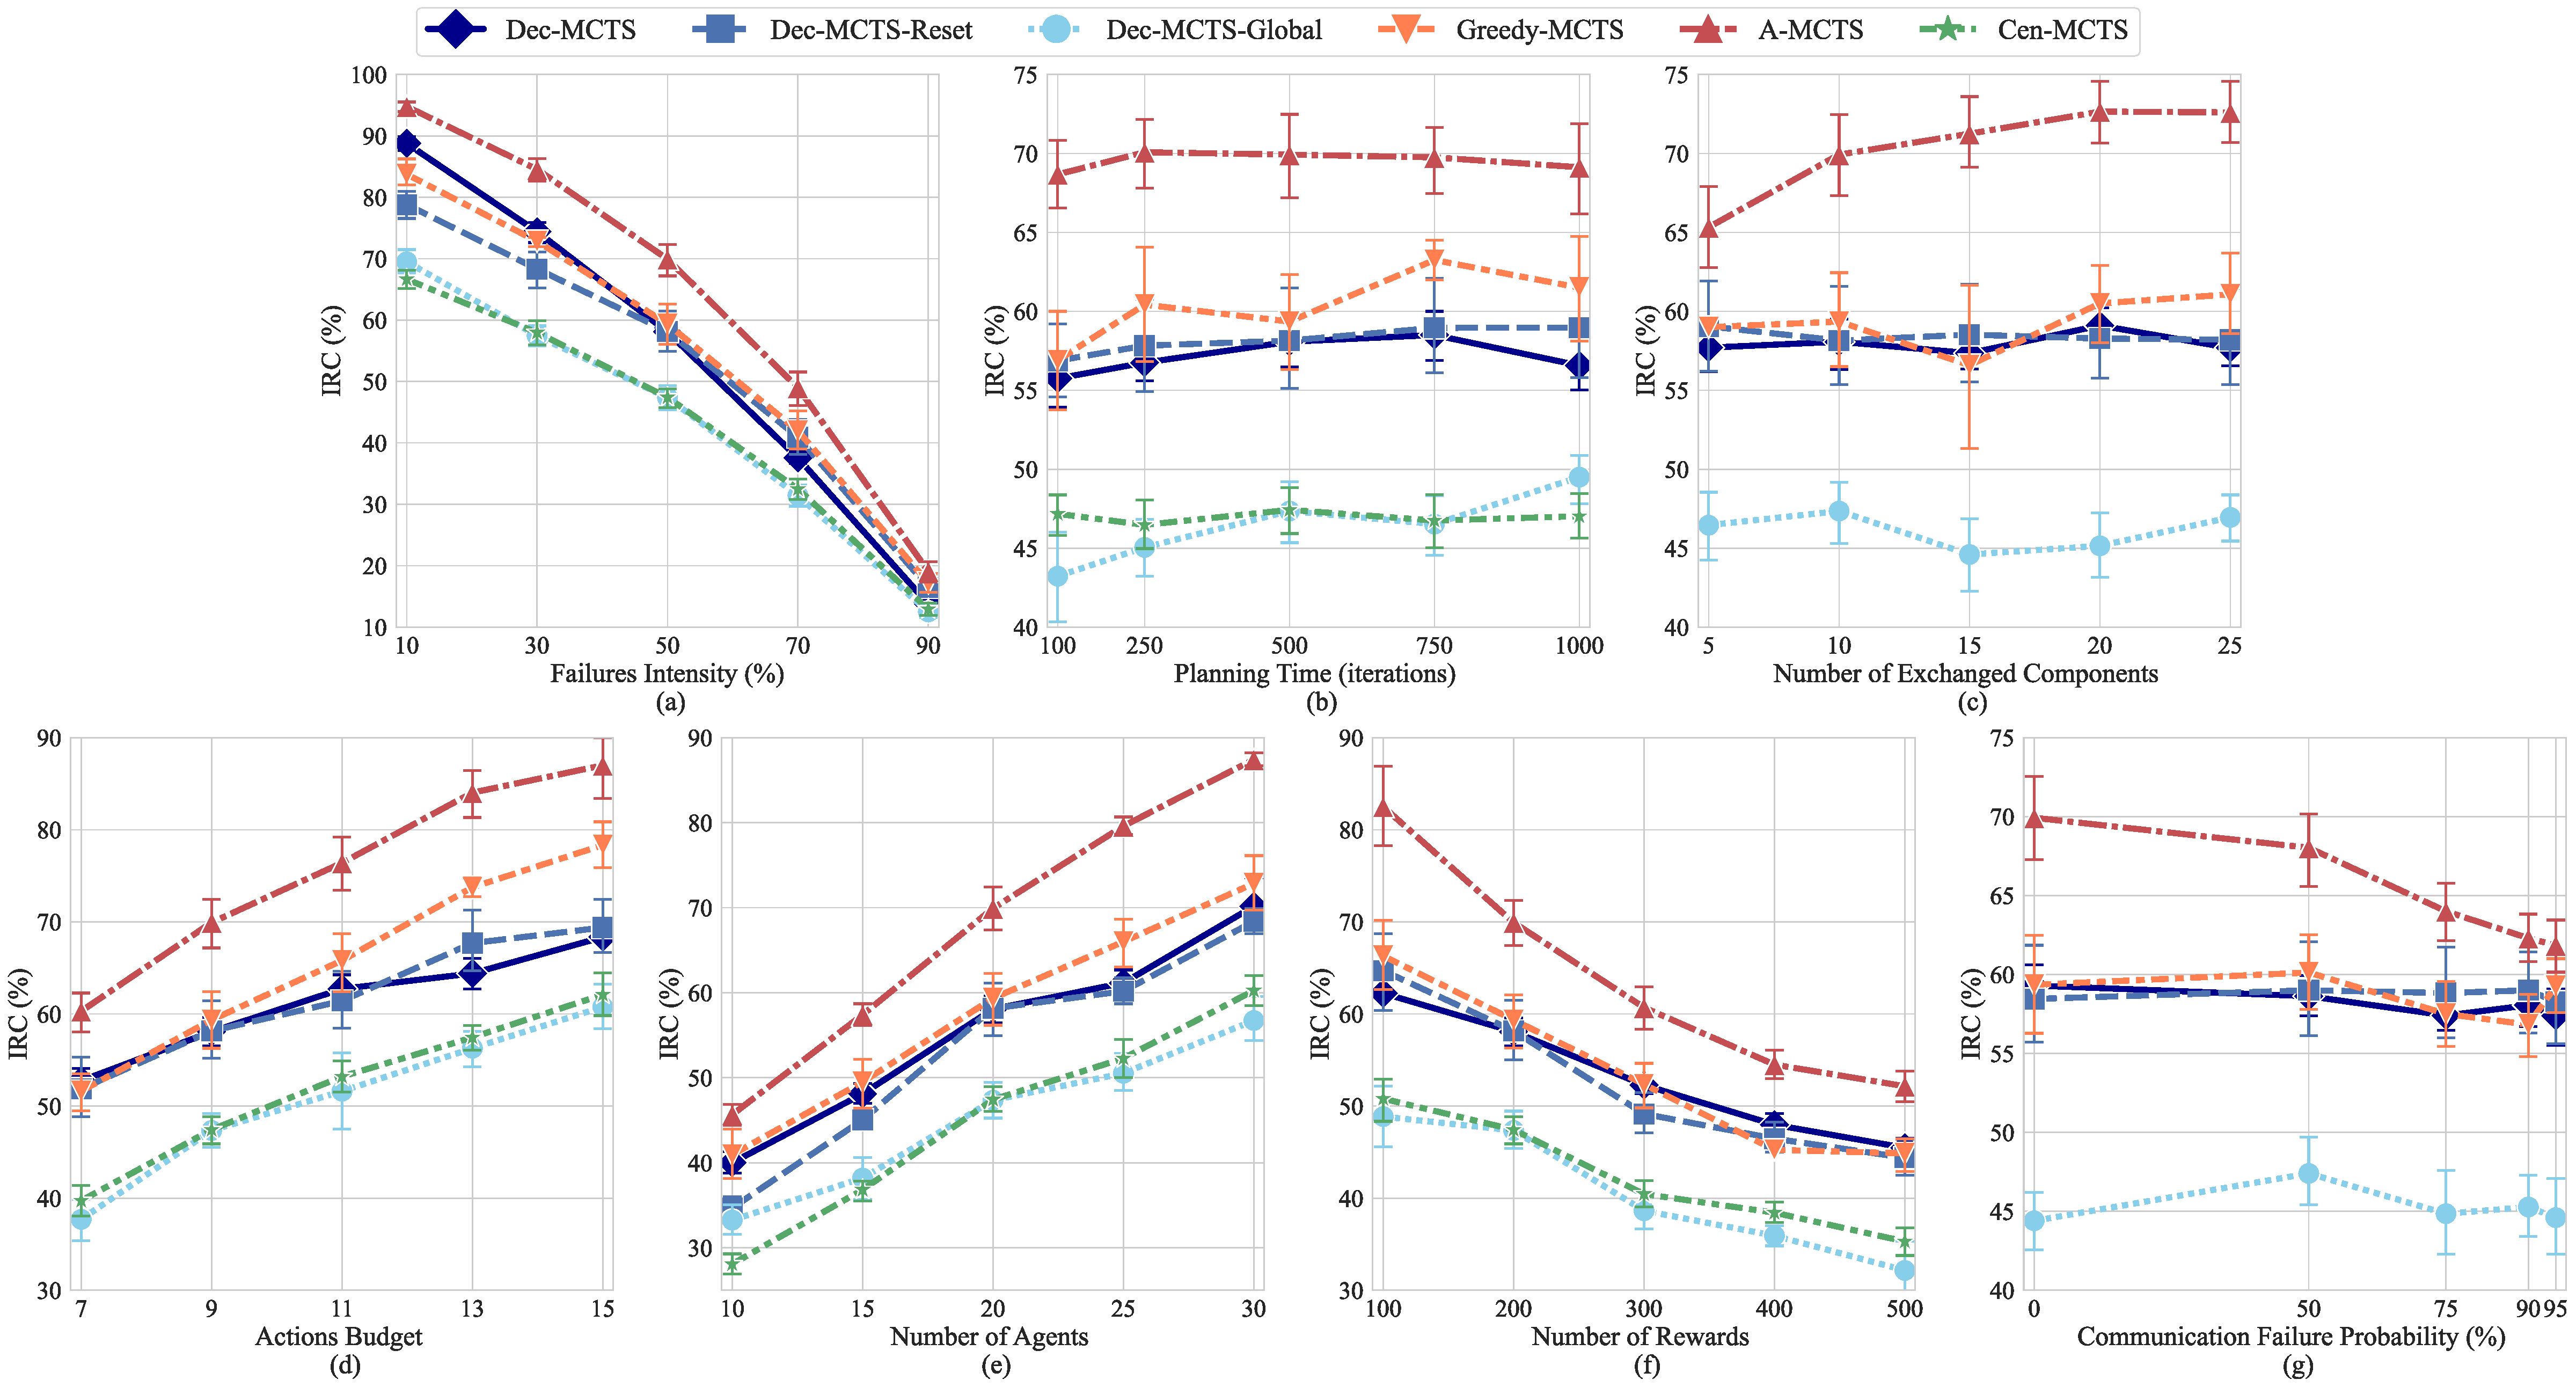
\includegraphics[width=\linewidth]{figs/stress.pdf}
		\caption{\footnotesize Impact of different parameters on the algorithms' performance at the mission end. Failures intensity (the fraction of agents that fail) (a); Planning time (b); Number of exchanged components (c); Actions budget (d), Number of agents (e); Number of rewards (f), and Communication failure probability (g). Results are with $95\%$ confidence interval.
        \label{fig:2}\normalsize 
        }
	\end{center}
\end{figure*}

To assess our A-MCTS algorithm, we consider the task of data collection from underwater wireless sensor networks (UWSN). Such tasks usually call for a collaboration of multiple autonomous underwater vehicles (AUVs) to traverse the environment and gather data from sensors.
The scenario consists of $200$ randomly distributed sensors in a $4000$ m $\times$ $4000$ m plane, with a transmission radius of $50$ m (typical for UWSN, e.g. \citep{cai2019data}). 
The graph $G$ of feasible paths is constructed using a probabilistic roadmap with a Dubins path model~\citep{kavraki1996probabilistic}. This model employs curves to refine the straight-line segments connecting waypoints and is extensively utilized for representing motion constraints pertinent to vehicle-like nonholonomic robots such as AUVs~\citep{41470}. The graph $G$ consists of $400$ vertices and an average of $19000$ edges.

We benchmark A-MCTS against the following baselines:
\begin{itemize}[leftmargin=*]
    \item \emph{Centralized MCTS (Central-MCTS)}: A single search tree is built for all of the $M$ harvesting agents with the actions of agent $m$ are at tree depth $(m, m + M, m + 2M,...)$.
    \item \emph{Dec-MCTS}~\citep{best2019dec}: It is the state-of-the-art decentralized multi-agent planning. In it, agents build their search tree with a marginal contribution utility function and adapt the same tree after churns occur.
    \item \emph{Dec-MCTS with reset (Dec-MCTS-Reset)}: Like Dec-MCTS, each agent builds its search tree with a marginal contribution utility function. Whenever churns occur, the tree of each agent is reset. This variant is considered to show that resetting the trees frequently could hamper the overall performance of the algorithm.
    \item \emph{Dec-MCTS with global utility (Dec-MCTS-Global}: Agents build their search tree with a global utility function and adapt the same tree after churns occur. This variant is considered to show that altering the utility function alone would not enhance performances against churns.
    \item \emph{A-MCTS with greedy optimization (Greedy-MCTS)}: In this scheme, we replace the RM Coordination (Algorithm 2) in our A-MCTS with a greedy algorithm, in which every agent sequentially picks the actions that deliver the highest immediate rewards for collaboration. This variant is considered to show that greedy solutions can be substantially suboptimal in MAS coordination.
\end{itemize}

For all algorithms, each planning phase consists of $500$ iterations, the discounting factor is set to $0.9$, and the exploration parameter is set to $0.4$ (i.e., within the ranges recommended in~\citep{best2019dec} to ensure the balance between exploration and exploitation). Unless otherwise stated, each agent compresses its tree into a set of $10$ possible paths and exchanges it with its teammates every $50$ planning iterations. Unless otherwise stated, we assume $20$ agents move in the graph, with a budget $B$ of $9$ actions. These values are chosen as they have proven to enable a high total utility score in the vast majority of scenarios considered in our experiments.

To model attrition in the population of agents, we assume that every agent has the same probability of failing during the mission and that the time at which each failure takes place is distributed uniformly at random throughout the mission duration. The key metric we use to evaluate the performance of the considered algorithms is the \emph{Instantaneous reward coverage (IRC)}, i.e. the fraction of available rewards covered (i.e. collected) at a given time.

\subsection{Performance Benchmarking}
In the first evaluation of our algorithm's adaptability to failures, we examine the impact of the failure intensity (i.e. fractions of agents that fail during the mission) on the IRC at the mission end, illustrated in Figure~\ref{fig:2}a. As expected, all algorithms experience performance declines with increasing intensity, reflecting reduced reward coverage due to fewer remaining agents in the system. Notably, with over $50\%$ of agents failing, Dec-MCTS-Reset surpasses the non-reset version due to the smaller system size which requires fewer iterations for exploration. Conversely, larger systems necessitate more time for agents to learn about the environment, hence frequent resets hamper the algorithm's performance.

To further elaborate on this matter, we assessed the impact of planning time on the IRC at the mission end. As Figure~\ref{fig:2}b shows, other baseline algorithms improved as planning time increased, with Dec-MCTS-Reset starting to outperform the non-reset with planning time larger than 750 iterations. A-MCTS, on the other hand, requires significantly less computational time yet still achieves the highest rewards regardless of the failure intensity and rates, thus proving itself as a good solution for online replanning.

The number of paths exchanged between agents significantly influences system complexity. Increased information exchange potentially leads to better algorithm performance, albeit at the expense of greater computational resources and time. To examine this trade-off, in Fig.~\ref{fig:2}c we evaluated the impact of different numbers of exchanged components on the IRC at the mission end. As expected, our proposed algorithm's performance improved with more exchanged components, while discounted algorithms showed no benefit. Indeed, with more exchanged components the utility of the joint policy found by regret matching improves too. However, given the finite number of optimal policies in a multi-agent game, escalating the number of components eventually yields diminishing returns.

As the above results show, resetting the tree would not consistently lead to improvement because the planning process involves initial exploration in which agents take random actions to learn reward distribution. Resetting without sufficient planning time results in suboptimal joint policies. Additionally, the use of the \emph{marginal contribution} utility combined with a \emph{submodular} reward function hampers agents' ability to recognize global reward reduction and hence adapt to failures efficiently. Moreover, sampling other agents' action sequences increases variance in global utility estimation and degrades the coordination quality. By assuming that the policies of other agents are fixed, A-MCTS can overcome this instability issue and adapt to agent failures better. Indeed, with regret matching aids in discovering better joint policies and thus provides better guidance for the exploration-exploitation of the search tree, our method exhibits superior performances in all cases.

In another set of experiments, we evaluated the impact of action budget $B$, the number of agents $N$, the number of rewards, and the communication failure probability, for a default failure intensity of $50\%$. As Fig. \ref{fig:2}d shows, A-MCTS managed to outperform Dec-MCTS substantially despite the difficulty of decentralized planning with a growing actions budget. Furthermore, as we doubled the budget of the action, the superiority of A-MCTS over the other techniques tripled. A similar behavior is exhibited by the system when we vary the number of agents. As shown in Fig.~\ref{fig:2}e, with a small number of agents, the differences between our algorithm and the discounted methods grow to $20\%$ with an increasing number of agents. In the considered settings, we also assess the impact of the density of sensors on the algorithms' performance by varying the number of sensors within the same area. As shown in Fig.~\ref{fig:2}f, the IRC declines as more sensors are introduced in the system. Naturally, with an increasing number of sensors the area that must be covered by agents expands as well. Nevertheless, A-MCTS shows better scalability as it consistently outperforms other methods.

The effectiveness of cooperative MAS is notably influenced by the quality of inter-agent communication. To understand better the impact of such limitations, we evaluated the algorithms' performances under different communication failure probabilities between each agent pair during a mission. As shown in Fig.~\ref{fig:2}g, there is no notable decline in A-MCTS performance even when half of the communication is disrupted, and it continues to outperform baseline methods with severely unstable communication. This highlights A-MCTS's ability to enable efficient cooperation among agents in hostile environments with restricted communication.

\subsection{Trade Off Between Communication Loss and Attrition for A-MCTS Analysis}

\begin{figure}[!ht]
	\begin{center}
        % \includesvg[width=\linewidth]{figs/tolerance.svg}
        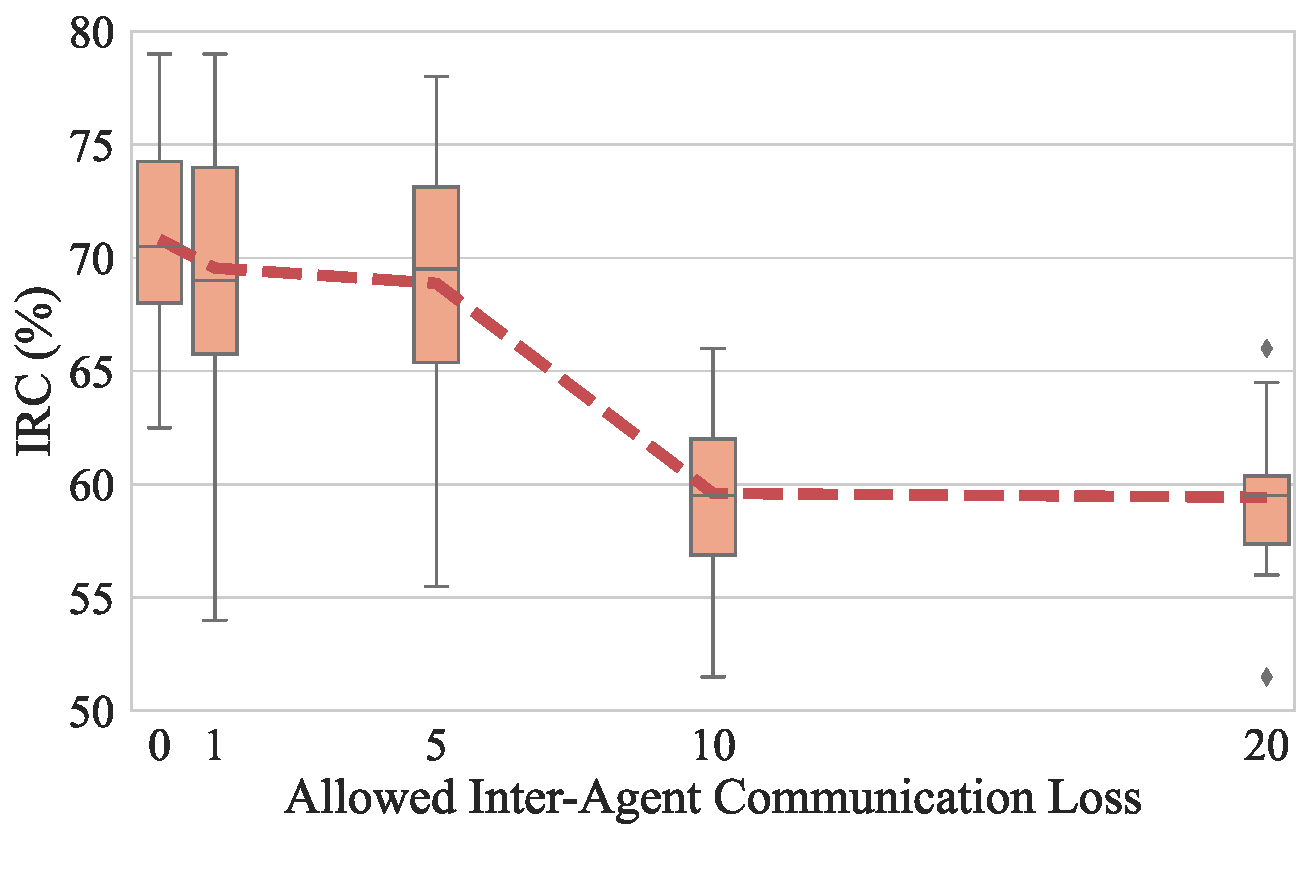
\includegraphics[width=\linewidth]{figs/tolerance.pdf}
		\caption{Impact of allowed inter-agent communication loss on the performance of A-MCTS at the end of the mission.
        \label{fig:a2}\normalsize}
	\end{center}
\end{figure}

In our approach, repeated communication loss is used as an indication of attrition. However, in practical settings, inter-agent communication can be unreliable and intermittent. If the algorithm is more sensitive to communication loss, it can mistakenly treat delayed messages as agent failures.

To better understand such impact, in this section, we study how tolerance to communication loss affects the performance of A-MCTS. Specifically, we parameterize this tolerance level by the number of times an agent must experience communication loss with another agent before treating it as attrition. Fig.~\ref{fig:a2} shows the IRC at the end of the mission against different numbers of allowed inter-agent communication loss. With up to 5 allowed messages loss, A-MCTS still shows no noticeable degradation. However, as the algorithm is more communication loss tolerant, the performance declines. This is expected because the remaining agents can not recognize churns fast enough and adapt efficiently.